\documentclass[10pt]{exam}
\usepackage[hon]{template-for-exam}
\usepackage{tikz,multicol}
\usetikzlibrary{arrows.meta}

\title{title}
\author{Rohrbach}
\date{\today}



\newcommand{\drawscantron}[2]{
  \begin{center}
    \begin{tikzpicture}
      %\node[anchor=south west] at (0,0) {
\includegraphics[width=6.4in]{49Q.png}};
      \fill (#1,#2) circle (0.25);
      \node at (9.5,19.5) {Physics Final Exam};
    \end{tikzpicture}

  \end{center}
}

\begin{document}

\newcommand{\printcontent}[1]{
  \vspace*{\stretch{1}}

  \begin{center}
    \Huge 
    
    \textbf{\sc Honors Physics}

    \textbf{\sc Fall Final Exam}

  \end{center}

  \begin{center}
    \Large (Version #1)
  \end{center}

  \vspace{2em}

  \begin{center}
    
      
\begin{tikzpicture}
        \draw (-0.3,0) -- (0.3,0) -- (0,0.530) -- cycle;
        \node at (0,0.2) {\bf !};
      \end{tikzpicture}
    
    
      {Please do not open this packet until instructed to do so!}
  \end{center}




  \paragraph{Rules} \hfill
  \begin{enumerate}
    \item \textbf{Phones, earbuds, headphones, smartwatches, computers, and other electronics must be put away in your backpacks against the wall during the entirety of the exam.  If electronics are out for \textit{any reason}, you will recieve a zero and a detention!}
    \item Put your name three places: On your Equation Sheet (back of this page), On your Scratch Work sheet (next page), and on the first page of the Exam Packet.
    \item Bubble in the Key Version (#1) on your Scantron
    \item When you are finished, turn in your scantron, equation sheet, and exam packet up front.
    \item Stay silent until all your classmates are finished.  Electronics (especially phones, but also earbuds, headphones, laptops, smartwatches, etc.) need to be kept away until the instructor indicates that everyone is finished.

  \end{enumerate}

  \vs[2]
}

\newcommand{\eqs}{
  {\noindent \LARGE \bf Equation Sheet}

  \section*{Basic Kinematics}

  \begin{align*}
    \bar{v} &\equiv \frac{\Delta x}{\Delta t} &
    \bar{a} &\equiv \frac{\Delta v}{\Delta t} &
    \bar{v} &= \frac{v+v_0}{2}
  \end{align*}


  \section*{Kinematic Equations}

  \vspace{-3em}

  \begin{multicols}{3}
    \begin{center}
    
        \begin{align*}
          v = v_0 + a t
        \end{align*}
        ``Old Faithful''
      
        \begin{align*}
          x = x_0 + v_0t + \frac{1}{2}at^2
        \end{align*}
        ``Big Chalupa''
      
        \begin{align*}
          v^2 = v_0^2 + 2a \left( x - x_0 \right)
        \end{align*}
        ``Ain't Got No Time''
    \end{center}
  \end{multicols}


  \section*{Range Equation}

  \begin{align*}
    R &= \frac{v_0^2 \sin\left(2\theta\right)}{g}
  \end{align*}

  \section*{Vectors \& Trig}

  \begin{minipage}{4in}
    \begin{center}
      \begin{align*}
        \sin{\theta} & =\frac{\text{opp}}{\text{hyp}} &
        \cos{\theta} & =\frac{\text{adj}}{\text{hyp}} &
        \tan{\theta} & =\frac{\text{opp}}{\text{adj}}
      \end{align*}
    \end{center}
  \end{minipage}
  %
  \begin{minipage}{2in}
    \begin{center}
      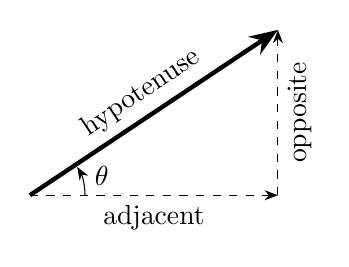
\begin{tikzpicture}[
        every node/.append style={},
        component/.append style={
          dashed,
          -{Stealth}
        },
        resultant/.append style={
          ultra thick,
          -{Stealth}
        },
        scale=0.7
    ]
      \draw[resultant] 
                (0,0) -- (4.5,3) 
                  node[midway,anchor=south,rotate=33.7]{hypotenuse};
      \draw[component] 
                (0,0) 
                -- (4.5,0) 
                  node[midway,anchor=north]{adjacent} ;
      \draw[component] 
                (4.5,0)
                -- (4.5,3) 
                  node[midway,anchor=north,rotate=90]{opposite} ;
      \draw[-Stealth] (1,0) node[anchor=south west]{$\theta$}
                arc[
                  start angle = 0,
                  end angle = 31, 
                  radius = 1
                ];
    \end{tikzpicture}


    \end{center}
  \end{minipage}


  \section*{Forces}

  \begin{align*}
    \Sigma F &= ma &
    w     &= mg &
    f_s  &= \mu_s N &
    f_k  &= \mu_k N
  \end{align*}

  \section*{Circular Motion \& Gravitation}

  \begin{align*}
    \Sigma F_C &= ma_C = \frac{mv^2}{r} &
    a_C        &= \frac{v^2}{r} &
    F_G        &= \frac{G m_1 m_2}{r^2} \\
    &&&& G     &= 
          \SI{6.67e-11}{\newton \meter^2\per\kilo\gram^2}
  \end{align*}

  \section*{Work \& Energy}

  \begin{align*}
    W    &= F_\parallel d = F d \cos\theta  &
    KE   &= \frac{1}{2} mv^2 &
    PE_g &= mgh &
    PE_e &= \frac{1}{2} kx^2
  \end{align*}

  \begin{align*}
    W &= \Delta KE &
    \Sigma E_0 + W_{NC} &= \Sigma E &
    P &= \frac{W}{t}
  \end{align*}
}


\printcontent{A}
\pagebreak
\eqs
\pagebreak 
\section*{Scratch Work} 
\pagebreak
\section*{Scratch Work} 
\pagebreak


\printcontent{B}
\pagebreak
\eqs
\pagebreak 
\section*{Scratch Work} 
\pagebreak
\section*{Scratch Work} 
\pagebreak


\printcontent{C}
\pagebreak
\eqs
\pagebreak 
\section*{Scratch Work} 
\pagebreak
\section*{Scratch Work} 
\pagebreak


\printcontent{D}
\pagebreak
\eqs
\pagebreak 
\section*{Scratch Work} 
\pagebreak
\section*{Scratch Work} 
\pagebreak





\end{document}